% !TeX program = xelatex
\documentclass[12pt,a4paper]{article}

\usepackage{fontspec}
\usepackage{polyglossia}
\setmainlanguage{russian}
\setmainfont{Liberation Serif}
\setmonofont{Noto Sans Mono}
\newfontfamily\cyrillicfonttt{Noto Sans Mono}
\usepackage{amsmath,amssymb,amsfonts}
\usepackage{graphicx}
\usepackage{geometry}
\usepackage{enumitem}
\usepackage{mathrsfs}
\usepackage{titlesec}
\usepackage{float}

\geometry{left=2.5cm,right=2.5cm,top=2cm,bottom=2cm}
\titleformat{\section}{\large\bfseries}{\thesection}{0.75em}{}
\titleformat{\subsection}{\normalsize\bfseries}{\thesubsection}{0.75em}{}
\DeclareMathSizes{12}{14}{10}{8}
\allowdisplaybreaks

\begin{document}

\begin{center}
    {\Large \textbf{Лабораторная работа 4.2}}\\[0.3em]
    {\Large \textbf{Тригонометрические ряды Фурье}}\\[0.3em]
    {\large Шерстобитов Евгений M3235}\\[0.3em]
    {\large Вариант 91}
\end{center}

\[
f(x)=[x], \quad x\in [0,3.5]
\]

\section{Аналитический метод}

\subsection{Исследование функции}

\subsubsection*{Общий тригонометрический ряд}

Известно, что
\[
f(x)\sim
\frac{a_0}{2}
+
\sum_{k=1}^{\infty}
\left(
a_k\cos\frac{\pi kx}{l}
+
b_k\sin\frac{\pi kx}{l}
\right)
\]

При условии, что $x\in [-l,l]$ \\

Пусть
\[
t=x-\frac{0+\frac72}{2}=x-\frac74
\]

Тогда
\[
t=x-\frac74\in\left[-\frac74,\frac74\right], \text{ при } x\in\left[0;\frac72\right]
\]

То есть $l=\frac74$

Определим функцию
\[
g(t)=f\left(t+\frac74\right),
\qquad
t\in\left[-\frac74;\frac74\right].
\]

Получаем, что
\[
g(t)\sim
\frac{a_0}{2} + \sum_{k=1}^{\infty}
\left(a_k\cos\frac{\pi kt}{l} + b_k\sin\frac{\pi kt}{l}
\right)
=
\frac{a_0}{2} + \sum_{k=1}^{\infty}
\left(
a_k\cos\frac{4\pi kt}{7} + b_k\sin\frac{4\pi kt}{7}
\right).
\]

где
\[
a_k=
\frac1l
\int_{-l}^{l}
g(t)\cos\frac{\pi kt}{l}\,dt,
\qquad
k\in\mathbb N\cup\{0\},
\]

\[
b_k=
\frac1l
\int_{-l}^{l}
g(t)\sin\frac{\pi kt}{l}\,dt,
\qquad
k\in\mathbb N
\]

Так как $t=x-\frac74$, то для исходной функции получаем
\[
f(x)=g\left(x-\frac74\right)
\]

Следовательно
\[
f(x)\sim \frac{a_0}{2} +
\sum_{k=1}^{\infty}
\left(
a_k\cos\frac{4\pi k\left(x-\frac74\right)}{7}
+
b_k\sin\frac{4\pi k\left(x-\frac74\right)}{7}
\right)
\]

\[
a_k=
\frac47
\int_{-7/4}^{7/4}
g(t)\cos\frac{4\pi kt}{7}\,dt,
\qquad k\in\mathbb N\cup\{0\},
\]

\[
b_k=
\frac47
\int_{-7/4}^{7/4}
g(t)\sin\frac{4\pi kt}{7}\,dt,
\qquad k\in\mathbb N.
\]

Значения функции \(g(t)\) на промежутке $\left[-\frac74,\frac74\right]$:

\[
g(t)=
\begin{cases}
0, & t\in\left[-\frac74,-\frac34\right) \\[2mm]
1, & t\in\left[-\frac34,\frac14\right) \\[2mm]
2, & t\in\left[\frac14,\frac54\right) \\[2mm]
3, & t\in\left[\frac54,\frac74\right]
\end{cases}
\]

Для \(k=0\):
\begin{align*}
a_0
&=
\frac47
\int_{-7/4}^{7/4}g(t)\,dt \\
&=
\frac47
\left(
\int_{-7/4}^{-3/4}0\,dt
+
\int_{-3/4}^{1/4}1\,dt
+
\int_{1/4}^{5/4}2\,dt
+
\int_{5/4}^{7/4}3\,dt
\right) \\
&=
\frac47
\left(
0
+
1\cdot\left(\frac14+\frac34\right)
+
2\cdot\left(\frac54-\frac14\right)
+
3\cdot\left(\frac74-\frac54\right)
\right) \\
&=
\frac47
\left(
1+2+\frac32
\right) \\
&=
\frac47\cdot\frac92
=
\frac{18}{7}
\end{align*}

Следовательно
\[
\frac{a_0}{2}=\frac97.
\]

Обозначим $ \alpha_k=\frac{4\pi k}{7} $. Тогда
\begin{align*}
a_k
&=
\frac47
\int_{-7/4}^{7/4}
g(t)\cos(\alpha_k t)\,dt = \\
&=
\frac47
\left(
\int_{-3/4}^{1/4}\cos(\alpha_k t)\,dt
+
2\int_{1/4}^{5/4}\cos(\alpha_k t)\,dt
+
3\int_{5/4}^{7/4}\cos(\alpha_k t)\,dt
\right) = \\
&=
\frac47
\left(
\frac{\sin\frac{\alpha_k}{4}-\sin\left(-\frac{3\alpha_k}{4}\right)}{\alpha_k}
+
2\frac{\sin\frac{5\alpha_k}{4}-\sin\frac{\alpha_k}{4}}{\alpha_k}
+
3\frac{\sin\frac{7\alpha_k}{4}-\sin\frac{5\alpha_k}{4}}{\alpha_k}
\right) = \\
&=
\frac4{7\alpha_k}
\left(
\sin\frac{\alpha_k}{4}
-
\sin\left(-\frac{3\alpha_k}{4}\right)
+
2\sin\frac{5\alpha_k}{4}
-
2\sin\frac{\alpha_k}{4}
+
3\sin\frac{7\alpha_k}{4}
-
3\sin\frac{5\alpha_k}{4}
\right) = \\
&=
\frac4{7\alpha_k}
\left(
-\sin\frac{\alpha_k}{4}
+
\sin\frac{3\alpha_k}{4}
-
\sin\frac{5\alpha_k}{4}
+
3\sin\frac{7\alpha_k}{4}
\right) = \\
&=
\frac4{7\alpha_k}
\left(
-\sin\frac{\alpha_k}{4}
+
\sin\frac{3\alpha_k}{4}
-
\sin\frac{5\alpha_k}{4}
+
3\sin(\pi k)
\right) = \\
&=
\frac4{7\alpha_k}
\left(
-\sin\frac{\alpha_k}{4}
+
\sin\frac{3\alpha_k}{4}
-
\sin\frac{5\alpha_k}{4}
\right) =
\frac1{\pi k}
\left(
-\sin\frac{\alpha_k}{4}
+
\sin\frac{3\alpha_k}{4}
-
\sin\frac{5\alpha_k}{4}
\right) = \\
&=
\frac{
-\sin\frac{\alpha_k}{4}
+
\sin\frac{3\alpha_k}{4}
-
\sin\frac{5\alpha_k}{4}
}{\pi k}
=
\frac{
-\sin\frac{\pi k}{7}
+
\sin\frac{3\pi k}{7}
-
\sin\frac{5\pi k}{7}
}{\pi k}
\end{align*}

Следовательно
\[
a_k
=
\frac{
-\sin\frac{\pi k}{7}
+
\sin\frac{3\pi k}{7}
-
\sin\frac{5\pi k}{7}
}{\pi k}
\]

Теперь вычислим $b_k$:

\begin{align*}
b_k
&=
\frac47
\int_{-7/4}^{7/4}
g(t)\sin(\alpha_k t)\,dt
= \\ &=
\frac47
\left(
\int_{-3/4}^{1/4}\sin(\alpha_k t)\,dt
+
2\int_{1/4}^{5/4}\sin(\alpha_k t)\,dt
+
3\int_{5/4}^{7/4}\sin(\alpha_k t)\,dt
\right)
= \\ &=
\frac47
\left(
\frac{
\cos\left(-\frac{3\alpha_k}{4}\right)
-
\cos\frac{\alpha_k}{4}
}{\alpha_k}
+
2\frac{
\cos\frac{\alpha_k}{4}
-
\cos\frac{5\alpha_k}{4}
}{\alpha_k}
+
3\frac{
\cos\frac{5\alpha_k}{4}
-
\cos\frac{7\alpha_k}{4}
}{\alpha_k}
\right)
= \\ &=
\frac4{7\alpha_k}
\left(
\cos\left(-\frac{3\alpha_k}{4}\right)
-
\cos\frac{\alpha_k}{4}
+
2\cos\frac{\alpha_k}{4}
-
2\cos\frac{5\alpha_k}{4}
+
3\cos\frac{5\alpha_k}{4}
-
3\cos\frac{7\alpha_k}{4}
\right)
= \\ &=
\frac4{7\alpha_k}
\left(
\cos\frac{\alpha_k}{4}
+
\cos\frac{3\alpha_k}{4}
+
\cos\frac{5\alpha_k}{4}
-
3\cos\frac{7\alpha_k}{4}
\right)
= \\ &=
\frac4{7\alpha_k}
\left(
\cos\frac{\alpha_k}{4}
+
\cos\frac{3\alpha_k}{4}
+
\cos\frac{5\alpha_k}{4}
-
3(-1)^k
\right)
= \\ &=
\frac{
\cos\frac{\alpha_k}{4}
+
\cos\frac{3\alpha_k}{4}
+
\cos\frac{5\alpha_k}{4}
-
3(-1)^k
}{\pi k}
=
\frac{
\cos\frac{\pi k}{7}
+
\cos\frac{3\pi k}{7}
+
\cos\frac{5\pi k}{7}
-
3(-1)^k
}{\pi k}
\end{align*}

Следовательно

\[
b_k
=
\frac{
\cos\frac{\pi k}{7}
+
\cos\frac{3\pi k}{7}
+
\cos\frac{5\pi k}{7}
-
3(-1)^k
}{\pi k}
\]

Итого имеем:
\[
f(x)\sim
\frac97
+
\sum_{k=1}^{\infty}
\left(
a_k\cos\frac{4\pi k\left(x-\frac74\right)}{7}
+
b_k\sin\frac{4\pi k\left(x-\frac74\right)}{7}
\right)
\]

где
\[
a_k=
\frac{
-\sin\frac{\pi k}{7}
+
\sin\frac{3\pi k}{7}
-
\sin\frac{5\pi k}{7}
}{\pi k},
\]
\[
b_k=
\frac{
\cos\frac{\pi k}{7}
+
\cos\frac{3\pi k}{7}
+
\cos\frac{5\pi k}{7}
-
3(-1)^k
}{\pi k}
\]

\subsubsection*{Сумма ряда}

Пусть
\[
y=\frac{\pi}{7/4}t=\frac{4\pi}{7}t
\]

Получаем, что
\[
t\in\left[-\frac74,\frac74\right]
\quad \Rightarrow \quad
y\in[-\pi,\pi].
\]

Определим функцию
\[
\varphi(y)=g\left(\frac{l}{\pi}y\right)
\]

Функция \(g\) кусочно постоянна и ограничена на $\left[-\frac74,\frac74\right]$

Следовательно, \(\varphi\) тоже кусочно постоянна и ограничена
на \([-\pi,\pi]\). Поэтому
\[
\varphi\in L^1[-\pi,\pi].
\]

Условие Гёльдера. Так как \(\varphi\) кусочно постоянна, то для любой точки \(y_0\)
существует такое \(\delta>0\), что при всех \(u\in(0,\delta)\)
справа и слева от точки \(y_0\) функция совпадает со своими
односторонними пределами:
\[
\varphi(y_0+u)=\varphi(y_0+0),
\qquad
\varphi(y_0-u)=\varphi(y_0-0).
\]

Следовательно,
\[
|\varphi(y_0+u)-\varphi(y_0+0)|=0,
\qquad
|\varphi(y_0-u)-\varphi(y_0-0)|=0.
\]

Значит, условие Гёльдера выполнено.

Тогда по теореме Дирихле ряд Фурье функции \(\varphi\) в точке \(y_0\) сходится к
\[
S_\varphi(y_0) = \frac{\varphi(y_0+0)+\varphi(y_0-0)}{2}
\]

При
\[
y_0=\frac{\pi}{l}t_0
\]

Имеем
\[
t_0=\frac{l}{\pi}y_0
\]

Поскольку
\[
\frac{l}{\pi}>0,
\]

Односторонние пределы сохраняют направление:
\[
\varphi(y_0+0)
=
g(t_0+0),
\]
\[
\varphi(y_0-0)
=
g(t_0-0).
\]

Следовательно, возвращаясь к переменной \(t\), получаем, что сумма ряда
Фурье функции \(g\) в точке \(t_0\) равна
\[
S(t_0)=
\frac{g(t_0+0)+g(t_0-0)}{2}.
\]

Функция \(g\) периодически продолжена с периодом
\[
2l=\frac72.
\]

На одном периоде $t\in\left[-\frac74,\frac74\right]$ имеем
\[
g(t)=
\begin{cases}
0, & t\in\left[-\frac74,-\frac34\right)\\[2mm]
1, & t\in\left[-\frac34,\frac14\right)\\[2mm]
2, & t\in\left[\frac14,\frac54\right)\\[2mm]
3, & t\in\left[\frac54,\frac74\right]
\end{cases}
\]

Следовательно, в точках непрерывности сумма ряда совпадает с функцией
\(g(t)\), а в точках разрыва равна полусумме левого и правого пределов.

Точки разрыва на одном периоде:
\[
t=-\frac74,\quad t=-\frac34,\quad t=\frac14,\quad t=\frac54,\quad t=\frac74.
\]

Поэтому
\[
S\left(-\frac34\right)=\frac{g(-\frac34 - 0) + g(- \frac34 + 0)}{2}=\frac{0+1}{2}=\frac12.
\]

\[
S\left(\frac14\right)=\frac{g(\frac14 - 0) + g(\frac14 + 0)}{2}=\frac{1+2}{2}=\frac32.
\]

\[
S\left(\frac54\right)=\frac{g(\frac54 - 0) + g(\frac54 + 0)}{2}=\frac{2+3}{2}=\frac52.
\]

\[
S\left(-\frac74\right)=S\left(\frac74\right)=\frac{3+0}{2}=\frac32.
\]

На одном периоде $t\in\left[-\frac74,\frac74\right]$ сумма ряда равна
\[
S(t)=
\begin{cases}
\frac32, & t=-\frac74,\\[2mm]
0, & -\frac74<t<-\frac34,\\[2mm]
\frac12, & t=-\frac34,\\[2mm]
1, & -\frac34<t<\frac14,\\[2mm]
\frac32, & t=\frac14,\\[2mm]
2, & \frac14<t<\frac54,\\[2mm]
\frac52, & t=\frac54,\\[2mm]
3, & \frac54<t<\frac74,\\[2mm]
\frac32, & t=\frac74.
\end{cases}
\]

Обратная замена:
\[
x=t+\frac74.
\]

Сумма ряда для одного периода $[0,\frac72]$:

\[
S(x)=
\begin{cases}
\frac32, & x=0,\\[2mm]
0, & 0<x<1,\\[2mm]
\frac12, & x=1,\\[2mm]
1, & 1<x<2,\\[2mm]
\frac32, & x=2,\\[2mm]
2, & 2<x<3,\\[2mm]
\frac52, & x=3,\\[2mm]
3, & 3<x<\frac72,\\[2mm]
\frac32, & x=\frac72
\end{cases}
\]

Теперь напишем сумму ряда для всех точек.

Так как сумма ряда периодична с периодом $T=\frac72$,
то для нахождения значения суммы при произвольном \(x\in\mathbb R\)
достаточно перейти к соответствующей точке одного периода.

Для этого положим
\[
r=x-T\left\lfloor \frac{x}{T}\right\rfloor
=
x-\frac72\left\lfloor \frac{x}{7/2}\right\rfloor
=
x-\frac72\left\lfloor \frac{2x}{7}\right\rfloor.
\]

Тогда
\[
r\in\left[0,\frac72\right).
\]

Из периодичности суммы следует, что
\[
S(x)=S(r).
\]

Поэтому сумма при всех \(x\in\mathbb R\):
\[
S(x)=
\begin{cases}
\frac32, & r=0,\\[2mm]
0, & 0<r<1,\\[2mm]
\frac12, & r=1,\\[2mm]
1, & 1<r<2,\\[2mm]
\frac32, & r=2,\\[2mm]
2, & 2<r<3,\\[2mm]
\frac52, & r=3,\\[2mm]
3, & 3<r<\frac72.
\end{cases}
\]

\subsubsection*{График суммы ряда}

На рисунке изображена сумма ряда Фурье \(S(x)\). Горизонтальные отрезки
соответствуют значениям суммы на интервалах
непрерывности функции. Отдельными точками отмечены значения суммы в
точках разрыва: в этих точках ряд принимает среднее арифметическое
левого и правого пределов функции.

Пунктирные вертикальные линии показывают границы периодов. Так как
период равен \(T=\frac72\), один и тот же вид графика повторяется на
каждом промежутке длины \(\frac72\).

\begin{figure}[h]
    \centering
    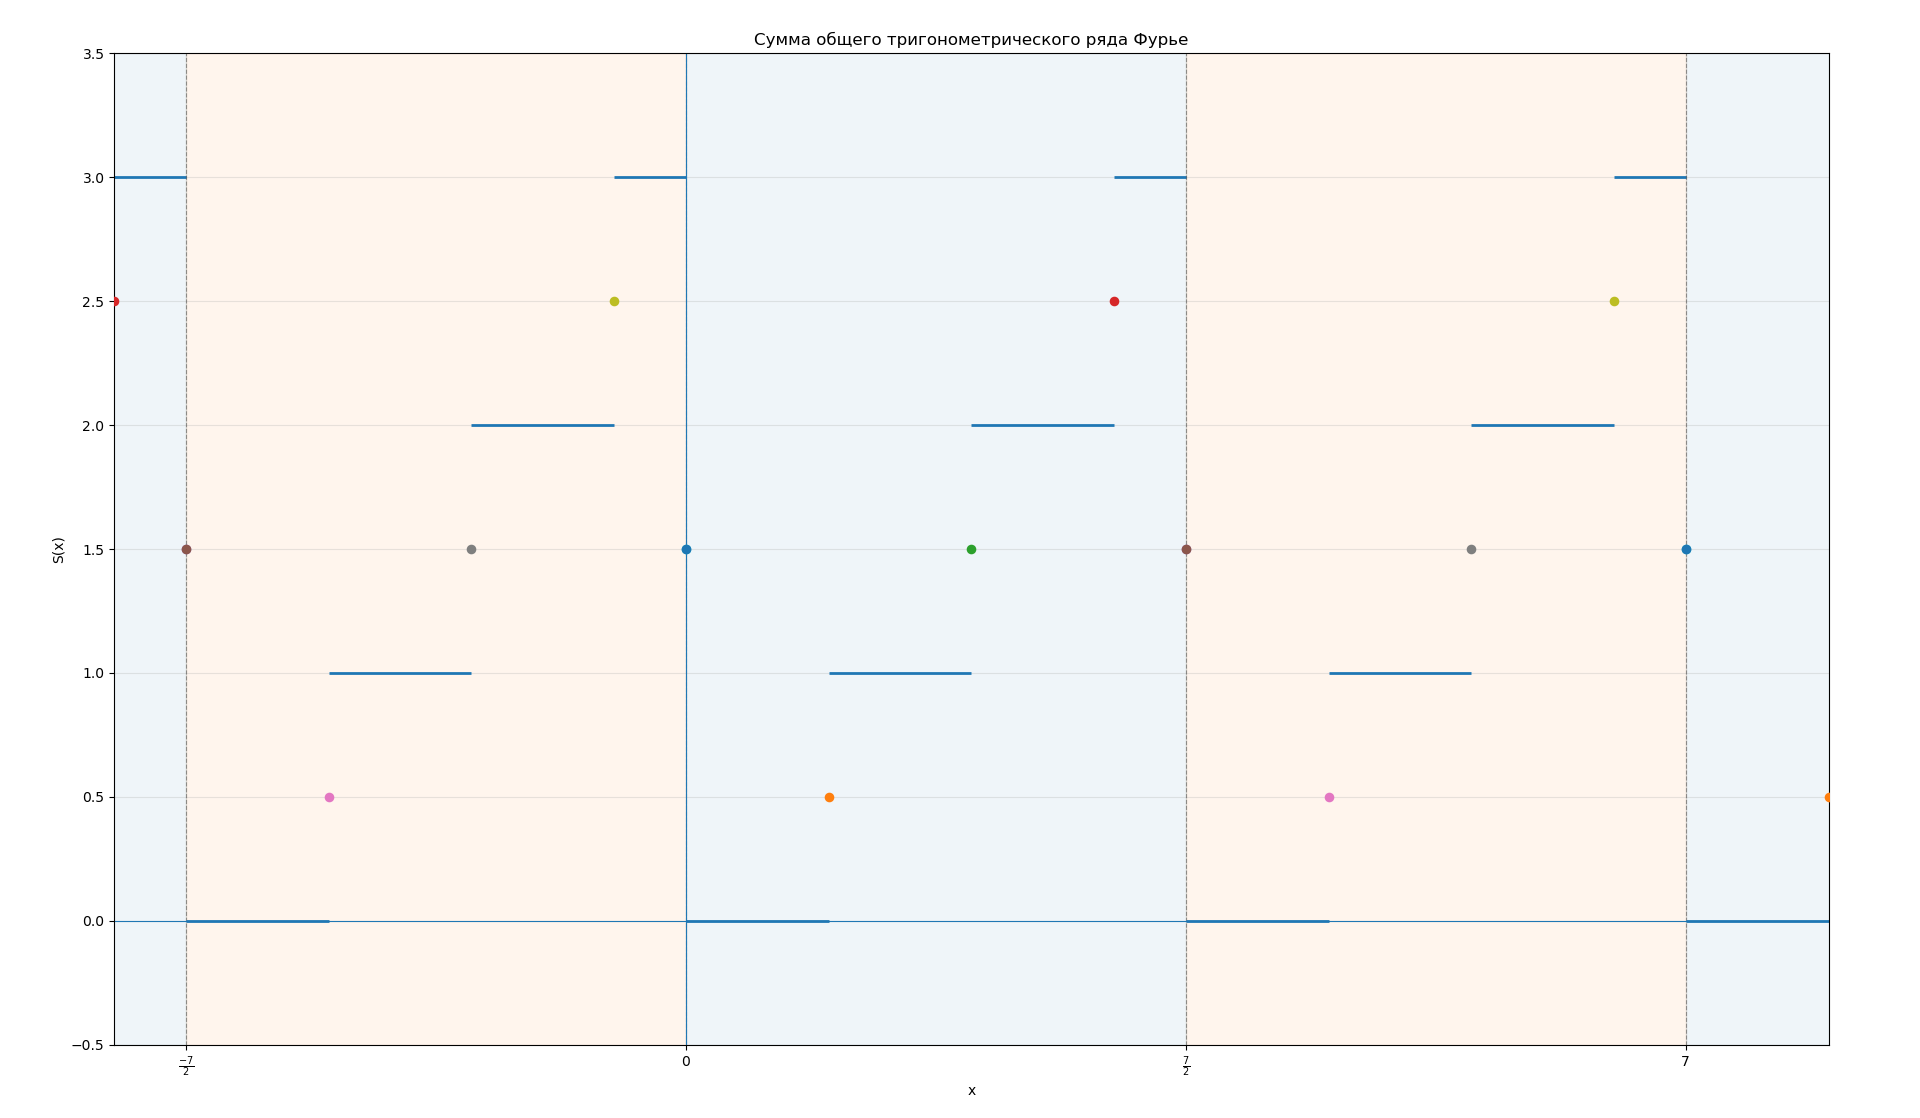
\includegraphics[width=1\textwidth]{../imgs/Figure_1.png}
    \caption{График суммы ряда}
\end{figure}

\subsection{Продолжение функции четным образом}

\subsubsection*{Ряд Фурье по косинусам}

Требуется продолжить функцию чётным образом.

Тогда симметричный промежуток имеет вид
\[
[-l,l]=\left[-\frac72,\frac72\right].
\]

Определим чётное продолжение функции \(f\) на этот промежуток. Обозначим
его через \(F_c\).
\[
F_c(x)=f(|x|)=[|x|].
\]

\begin{align*}
F_c(x)&\sim
\frac{a_0}{2}
+
\sum_{k=1}^{\infty}
\left(
a_k\cos\frac{\pi kx}{l}
+
b_k\sin\frac{\pi kx}{l}
\right)
= \\ &=
\frac{a_0}{2}
+
\sum_{k=1}^{\infty}
\left(
a_k\cos\frac{2\pi kx}{7}
+
b_k\sin\frac{2\pi kx}{7}
\right)
\end{align*}

Так как \(F_c\) чётная и
\[
\sin\frac{2\pi kx}{7}
\]

нечетная, то их произведение
является нечётной функцией.

Следовательно
\[
b_k=
\frac1l
\int_{-l}^{l}
F_c(x)\sin\frac{\pi kx}{l}\,dx
=
0.
\]

Получаем
\[
F_c(x)\sim
\frac{a_0}{2}
+
\sum_{k=1}^{\infty}
a_k\cos\frac{2\pi kx}{7}.
\]

Так как \(F_c\) чётная, то коэффициенты \(a_k\) можно считать по формуле
\begin{align*}
a_k
&=
\frac{2}{l}
\int_0^l
f(x)\cos\frac{\pi kx}{l}\,dx
=
\frac47
\int_0^{7/2}
f(x)\cos\frac{2\pi kx}{7}\,dx
\end{align*}

Обозначим
\[
\alpha_k=\frac{2\pi k}{7}.
\]

Для \(k=0\):
\begin{align*}
a_0&=
\frac47
\int_0^{7/2}f(x)\,dx
=
\frac47
\left(
\int_0^1 0\,dx
+
\int_1^2 1\,dx
+
\int_2^3 2\,dx
+
\int_3^{7/2} 3\,dx
\right)
= \\ &=
\frac47
\left(
0+1+2+\frac32
\right)
=
\frac47\cdot\frac92
=
\frac{18}{7}.
\end{align*}

Следовательно,
\[
\frac{a_0}{2}=\frac97.
\]

Теперь вычислим $a_k$:

\begin{align*}
a_k&=
\frac47
\int_0^{7/2}
f(x)\cos(\alpha_k x)\,dx
= \\ &=
\frac47
\left(
\int_1^2 \cos(\alpha_kx)\,dx
+
2\int_2^3 \cos(\alpha_kx)\,dx
+
3\int_3^{7/2} \cos(\alpha_kx)\,dx
\right)
= \\ &=
\frac47
\left(
\frac{\sin(2\alpha_k)-\sin(\alpha_k)}{\alpha_k}
+
2\frac{\sin(3\alpha_k)-\sin(2\alpha_k)}{\alpha_k}
+
3\frac{\sin\left(\frac72\alpha_k\right)-\sin(3\alpha_k)}{\alpha_k}
\right)
= \\ &=
\frac4{7\alpha_k}
\left(
\sin(2\alpha_k)-\sin(\alpha_k)
+
2\sin(3\alpha_k)-2\sin(2\alpha_k)
+
3\sin\left(\frac72\alpha_k\right)-3\sin(3\alpha_k)
\right)
= \\ &=
\frac4{7\alpha_k}
\left(
-\sin(\alpha_k)
-\sin(2\alpha_k)
-\sin(3\alpha_k)
+
3\sin\left(\frac72\alpha_k\right)
\right)
= \\ &=
-\frac2{\pi k}
\left(
\sin(\alpha_k)
+
\sin(2\alpha_k)
+
\sin(3\alpha_k)
\right)
=
-\frac2{\pi k}
\left(
\sin\frac{2\pi k}{7}
+
\sin\frac{4\pi k}{7}
+
\sin\frac{6\pi k}{7}
\right).
\end{align*}

Получаем
\[
a_k=
-\frac2{\pi k}
\left(
\sin\frac{2\pi k}{7}
+
\sin\frac{4\pi k}{7}
+
\sin\frac{6\pi k}{7}
\right).
\]

Итого
\[
F_c(x)\sim
\frac97
-
\sum_{k=1}^{\infty}
\frac2{\pi k}
\left(
\sin\frac{2\pi k}{7}
+
\sin\frac{4\pi k}{7}
+
\sin\frac{6\pi k}{7}
\right)
\cos\frac{2\pi kx}{7}
\]

\subsubsection*{Сумма ряда по косинусам}

Функция \(F_c\) задана на промежутке
\[
\left[-\frac72,\frac72\right]
\]

Аналогично прошлому пункту определим функцию
\[
\varphi(y)=F_c\left(\frac{l}{\pi}y\right)
\]

Функция \(\varphi\) кусочно постоянна и ограничена на \([-\pi,\pi]\),
поэтому
\[
\varphi\in L^1[-\pi,\pi].
\]

Кроме того, функция \(\varphi\) кусочно постоянна, значит в каждой точке
существуют конечные односторонние пределы. Для достаточно малых \(u>0\)
справа и слева от каждой точки функция совпадает со своими односторонними
пределами, поэтому
\[
|\varphi(y_0+u)-\varphi(y_0+0)|=0,
\]
\[
|\varphi(y_0-u)-\varphi(y_0-0)|=0
\]

Следовательно, условие Гёльдера выполнено.

По теореме Дирихле ряд Фурье функции \(\varphi\) в точке \(y_0\) сходится к
\[
\frac{\varphi(y_0+0)+\varphi(y_0-0)}{2}
\]

Возвращаясь к переменной \(x\), получаем, что сумма ряда Фурье функции
\(F_c\) в точке \(x_0\) равна
\[
S_c(x_0)=
\frac{F_c(x_0+0)+F_c(x_0-0)}{2}
\]

На одном периоде
\[
x\in\left[-\frac72,\frac72\right]
\]

точками разрыва являются
\[
x=\pm1,\qquad x=\pm2,\qquad x=\pm3
\]

В точках непрерывности сумма ряда совпадает с \(F_c(x)\).

В точках разрыва:

Тогда
\[
S_c(\pm 1)=
\frac{F_c(\pm 1-0)+F_c(\pm 1+0)}{2}
=
\frac{0+1}{2}
=
\frac12
\]

\[
S_c(\pm 2)=
\frac{F_c(\pm 2-0)+F_c(\pm 2+0)}{2}
=
\frac{1+2}{2}
=
\frac32
\]

\[
S_c(\pm 3)=
\frac{F_c(\pm 3-0)+F_c(\pm 3+0)}{2}
=
\frac{2+3}{2}
=
\frac52
\]
\[
S_c(\pm \frac72)=
\frac{
F_c(\pm \frac72-0)
+
F_c(\pm \frac72+0)
}{2}
=
\frac{3+3}{2}
=
3
\]

Следовательно, на одном периоде
\[
x\in\left[-\frac72,\frac72\right]
\]
сумма ряда равна
\[
S_c(x)=
\begin{cases}
0, & |x|<1,\\[2mm]
\frac12, & |x|=1,\\[2mm]
1, & 1<|x|<2,\\[2mm]
\frac32, & |x|=2,\\[2mm]
2, & 2<|x|<3,\\[2mm]
\frac52, & |x|=3,\\[2mm]
3, & 3<|x|\le \frac72.
\end{cases}
\]

Чтобы записать сумму при всех \(x\in\mathbb R\), перенесём произвольную
точку \(x\) в основной период
\[
\left[-\frac72,\frac72\right)
\]

Положим
\[
r=x-7\left\lfloor\frac{x+\frac72}{7}\right\rfloor
\]

Тогда
\[
r\in\left[-\frac72,\frac72\right)
\]

Из периодичности следует, что
\[
S_c(x)=S_c(r).
\]

Поэтому при всех \(x\in\mathbb R\)
\[
S_c(x)=
\begin{cases}
0, & |r|<1,\\[2mm]
\frac12, & |r|=1,\\[2mm]
1, & 1<|r|<2,\\[2mm]
\frac32, & |r|=2,\\[2mm]
2, & 2<|r|<3,\\[2mm]
\frac52, & |r|=3,\\[2mm]
3, & 3<|r|\le \frac72.
\end{cases}
\]

\subsubsection*{График суммы ряда по косинусам}

Аналогично первому пункту изобразим график суммы ряда Фурье по косинусам

\begin{figure}[h]
    \centering
    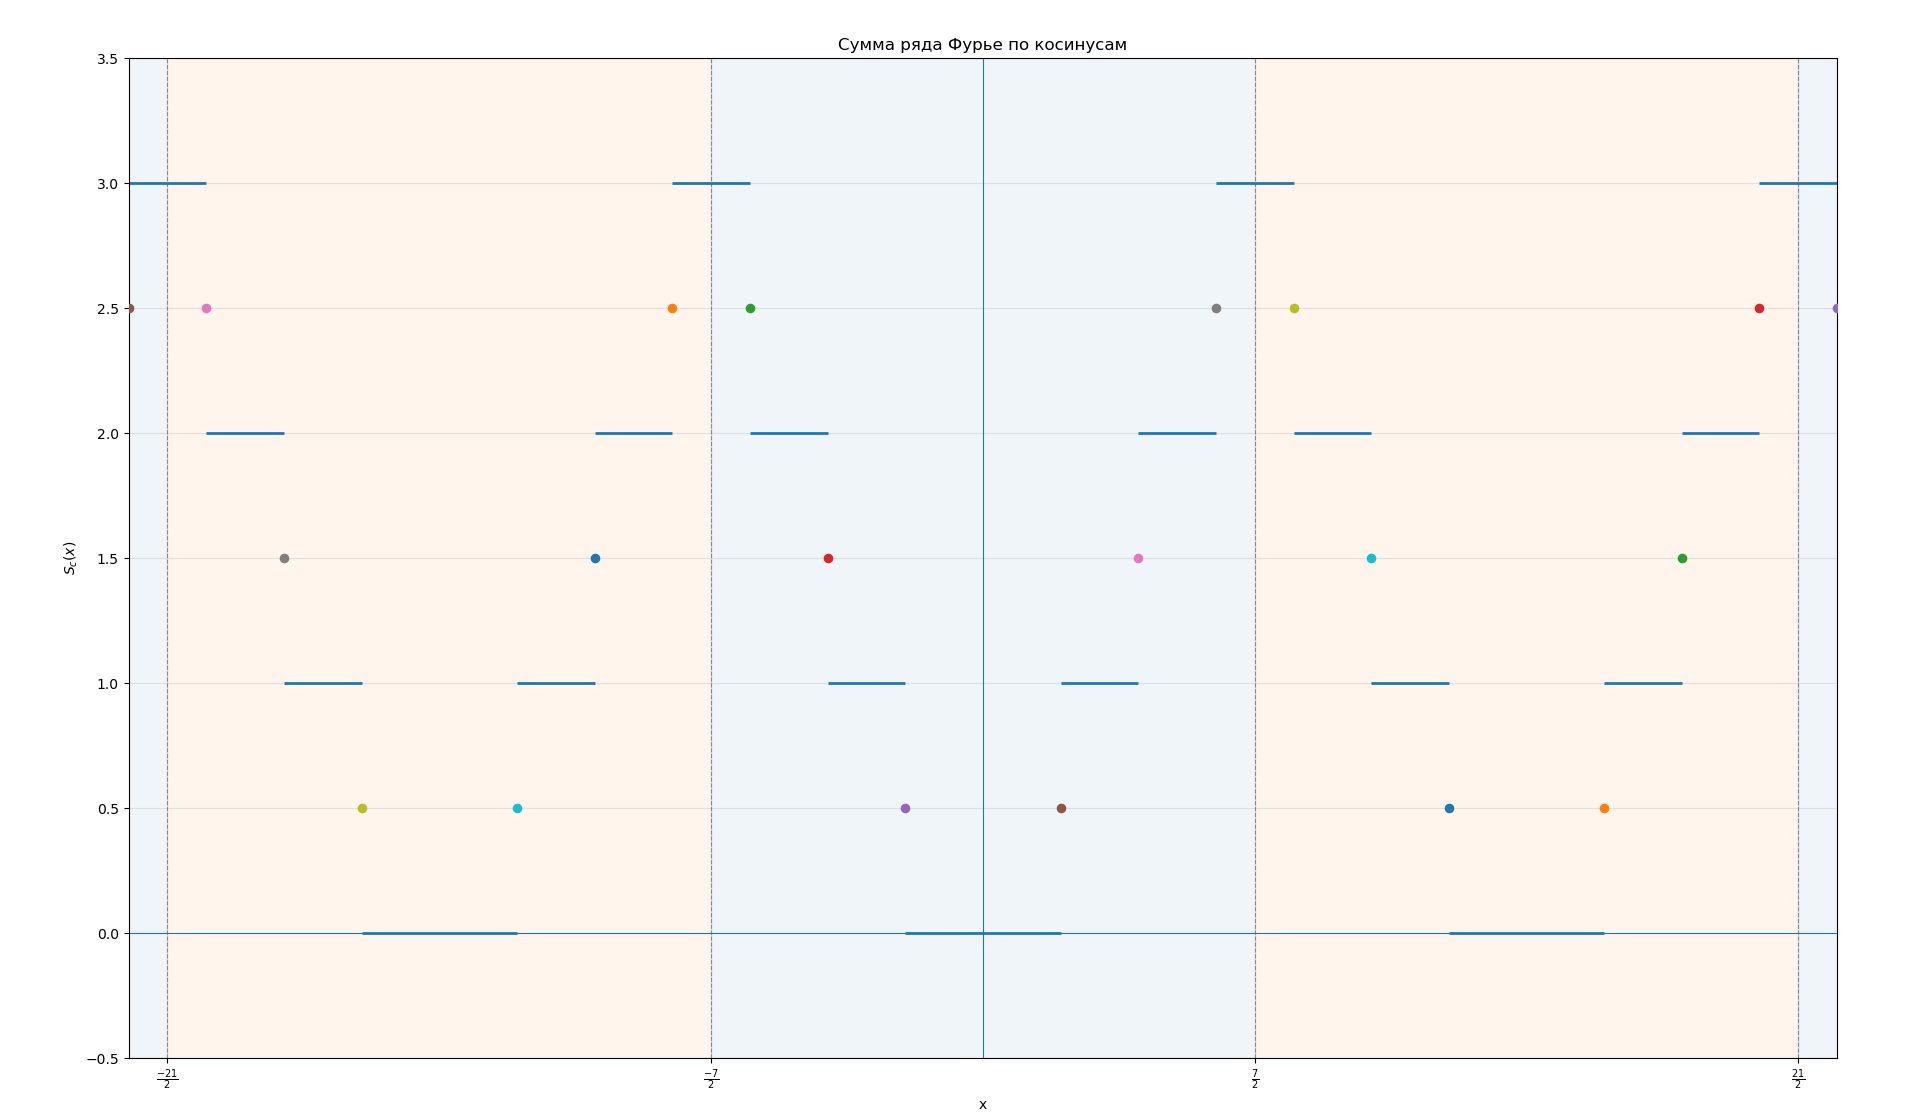
\includegraphics[width=1\textwidth]{../imgs/Figure_2.png}
    \caption{График суммы ряда Фурье по косинусам}
\end{figure}

\subsection{Продолжение функции нечетным образом}

\subsubsection*{Ряд Фурье по синусам}

Требуется продолжить функцию нечётным образом.

Тогда симметричный промежуток имеет вид
\[
[-l,l]=\left[-\frac72,\frac72\right].
\]

Определим нечётное продолжение функции \(f\) на этот промежуток. Обозначим
его через \(F_s\).
\[
F_s(x)=\operatorname{sgn}(x)f(|x|)
=
\operatorname{sgn}(x)[|x|].
\]

\begin{align*}
F_s(x)&\sim
\frac{a_0}{2}
+
\sum_{k=1}^{\infty}
\left(
a_k\cos\frac{\pi kx}{l}
+
b_k\sin\frac{\pi kx}{l}
\right)
= \\ &=
\frac{a_0}{2}
+
\sum_{k=1}^{\infty}
\left(
a_k\cos\frac{2\pi kx}{7}
+
b_k\sin\frac{2\pi kx}{7}
\right)
\end{align*}

Так как \(F_s\) нечётная, то
\[
a_0=
\frac1l
\int_{-l}^{l}
F_s(x)\,dx
=
0.
\]

Кроме того, \(F_s\) нечётная и
\[
\cos\frac{2\pi kx}{7}
\]

чётная, поэтому их произведение является нечётной функцией.

Следовательно
\[
a_k=
\frac1l
\int_{-l}^{l}
F_s(x)\cos\frac{\pi kx}{l}\,dx
=
0.
\]

Получаем
\[
F_s(x)\sim
\sum_{k=1}^{\infty}
b_k\sin\frac{2\pi kx}{7}.
\]

Посчитаем $b_k$:
\begin{align*}
b_k
&=
\frac{2}{l}
\int_0^l
f(x)\sin\frac{\pi kx}{l}\,dx
=
\frac47
\int_0^{7/2}
f(x)\sin\frac{2\pi kx}{7}\,dx
\end{align*}

Обозначим
\[
\alpha_k=\frac{2\pi k}{7}.
\]

Теперь вычислим \(b_k\):

\begin{align*}
b_k&=
\frac47
\int_0^{7/2}
f(x)\sin(\alpha_k x)\,dx
= \\ &=
\frac47
\left(
\int_1^2 \sin(\alpha_kx)\,dx
+
2\int_2^3 \sin(\alpha_kx)\,dx
+
3\int_3^{7/2} \sin(\alpha_kx)\,dx
\right)
= \\ &=
\frac47
\left(
\frac{\cos(\alpha_k)-\cos(2\alpha_k)}{\alpha_k}
+
2\frac{\cos(2\alpha_k)-\cos(3\alpha_k)}{\alpha_k}
+
3\frac{\cos(3\alpha_k)-\cos\left(\frac72\alpha_k\right)}{\alpha_k}
\right)
= \\ &=
\frac4{7\alpha_k}
\left(
\cos(\alpha_k)-\cos(2\alpha_k)
+
2\cos(2\alpha_k)-2\cos(3\alpha_k)
+
3\cos(3\alpha_k)-3\cos\left(\frac72\alpha_k\right)
\right)
= \\ &=
\frac4{7\alpha_k}
\left(
\cos(\alpha_k)
+
\cos(2\alpha_k)
+
\cos(3\alpha_k)
-
3\cos\left(\frac72\alpha_k\right)
\right)
= \\ &=
\frac2{\pi k}
\left(
\cos(\alpha_k)
+
\cos(2\alpha_k)
+
\cos(3\alpha_k)
-
3(-1)^k
\right)
= \\ &=
\frac2{\pi k}
\left(
\cos\frac{2\pi k}{7}
+
\cos\frac{4\pi k}{7}
+
\cos\frac{6\pi k}{7}
-
3(-1)^k
\right)
\end{align*}

Итого
\[
F_s(x)\sim
\sum_{k=1}^{\infty}
\frac2{\pi k}
\left(
\cos\frac{2\pi k}{7}
+
\cos\frac{4\pi k}{7}
+
\cos\frac{6\pi k}{7}
-
3(-1)^k
\right)
\sin\frac{2\pi kx}{7}
\]

\subsubsection*{Сумма ряда по синусам}

Функция \(F_s\) задана на промежутке
\[
\left[-\frac72,\frac72\right]
\]

Аналогично прошлому пункту определим функцию
\[
\varphi(y)=F_s\left(\frac{l}{\pi}y\right)
\]

Функция \(\varphi\) кусочно постоянна и ограничена на \([-\pi,\pi]\),
поэтому
\[
\varphi\in L^1[-\pi,\pi].
\]

Кроме того, функция \(\varphi\) кусочно постоянна, значит в каждой точке
существуют конечные односторонние пределы. Для достаточно малых \(u>0\)
справа и слева от каждой точки функция совпадает со своими односторонними
пределами, поэтому
\[
|\varphi(y_0+u)-\varphi(y_0+0)|=0,
\]
\[
|\varphi(y_0-u)-\varphi(y_0-0)|=0
\]

Следовательно, условие Гёльдера выполнено.

По теореме Дирихле ряд Фурье функции \(\varphi\) в точке \(y_0\) сходится к
\[
\frac{\varphi(y_0+0)+\varphi(y_0-0)}{2}
\]

Возвращаясь к переменной \(x\), получаем, что сумма ряда Фурье функции
\(F_s\) в точке \(x_0\) равна
\[
S_s(x_0)=
\frac{F_s(x_0+0)+F_s(x_0-0)}{2}
\]

На одном периоде
\[
x\in\left[-\frac72,\frac72\right]
\]

точками разрыва являются
\[
x=\pm1,\qquad x=\pm2,\qquad x=\pm3,\qquad x=\pm\frac72
\]

В точках непрерывности сумма ряда совпадает с \(F_s(x)\).

В точках разрыва:

Тогда
\[
S_s(\pm 1)=
\frac{F_s(\pm 1-0)+F_s(\pm 1+0)}{2}
=
\pm\frac{0+1}{2}
=
\pm\frac12
\]

\[
S_s(\pm 2)=
\frac{F_s(\pm 2-0)+F_s(\pm 2+0)}{2}
=
\pm\frac{1+2}{2}
=
\pm\frac32
\]

\[
S_s(\pm 3)=
\frac{F_s(\pm 3-0)+F_s(\pm 3+0)}{2}
=
\pm\frac{2+3}{2}
=
\pm\frac52
\]

В концах периода при периодическом продолжении односторонние пределы
равны \(3\) и \(-3\), поэтому
\[
S_s\left(\pm\frac72\right)=
\frac{3+(-3)}{2}
=
0.
\]

Следовательно, на одном периоде
\[
x\in\left[-\frac72,\frac72\right]
\]

сумма ряда равна
\[
S_s(x)=
\begin{cases}
0, & |x|<1,\\[2mm]
\frac12\operatorname{sgn}x, & |x|=1,\\[2mm]
\operatorname{sgn}x, & 1<|x|<2,\\[2mm]
\frac32\operatorname{sgn}x, & |x|=2,\\[2mm]
2\operatorname{sgn}x, & 2<|x|<3,\\[2mm]
\frac52\operatorname{sgn}x, & |x|=3,\\[2mm]
3\operatorname{sgn}x, & 3<|x|<\frac72,\\[2mm]
0, & |x|=\frac72.
\end{cases}
\]

Чтобы записать сумму при всех \(x\in\mathbb R\), перенесём произвольную
точку \(x\) в основной период
\[
\left[-\frac72,\frac72\right)
\]

Положим
\[
r=x-7\left\lfloor\frac{x+\frac72}{7}\right\rfloor
\]

Тогда
\[
r\in\left[-\frac72,\frac72\right)
\]

Из периодичности следует, что
\[
S_s(x)=S_s(r).
\]

Поэтому при всех \(x\in\mathbb R\)
\[
S_s(x)=
\begin{cases}
0, & |r|<1,\\[2mm]
\frac12\operatorname{sgn}r, & |r|=1,\\[2mm]
\operatorname{sgn}r, & 1<|r|<2,\\[2mm]
\frac32\operatorname{sgn}r, & |r|=2,\\[2mm]
2\operatorname{sgn}r, & 2<|r|<3,\\[2mm]
\frac52\operatorname{sgn}r, & |r|=3,\\[2mm]
3\operatorname{sgn}r, & 3<|r|<\frac72,\\[2mm]
0, & |r|=\frac72.
\end{cases}
\]

\newpage

\subsubsection*{График суммы ряда по синусам}

Аналогично первому пункту изобразим график суммы ряда Фурье по синусам.
Так как функция была продолжена нечётным образом, график симметричен
относительно начала координат.

\begin{figure}[h]
    \centering
    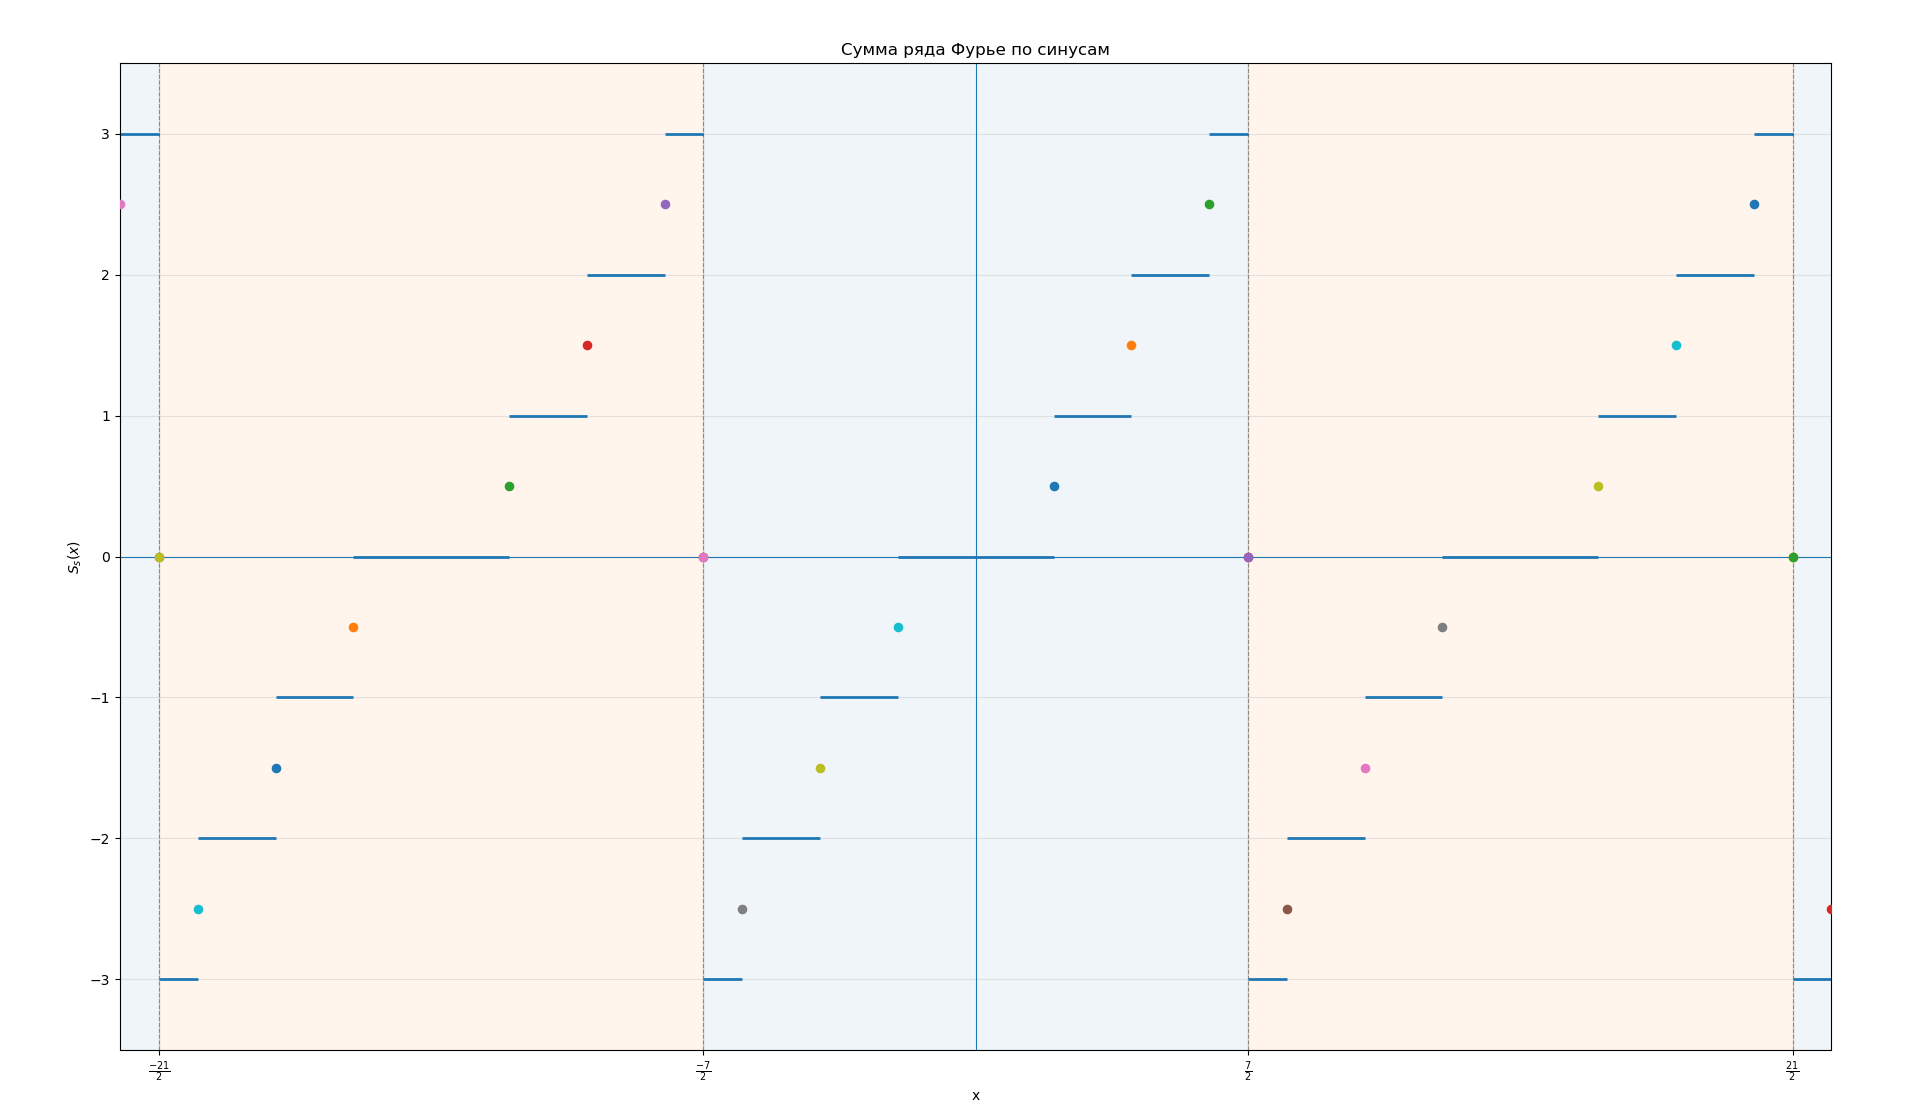
\includegraphics[width=1\textwidth]{../imgs/Figure_3.png}
    \caption{График суммы ряда Фурье по синусам}
\end{figure}

\section{Численный метод}

\subsection{Графики частичных сумм рядов}

Построим графики частичных сумм для трёх рядов, полученных в первой
части: общего тригонометрического ряда, ряда по синусам и ряда по
косинусам. Для каждого ряда рассмотрим несколько значений числа
слагаемых:
\[
N=3,\qquad N=10,\qquad N=30.
\]

\subsubsection*{Общий ряд}

Для общего тригонометрического ряда частичная сумма имеет вид
\[
S_n(x)=
\frac97
+
\sum_{k=1}^{n}
\left(
a_k\cos\frac{4\pi k\left(x-\frac74\right)}{7}
+
b_k\sin\frac{4\pi k\left(x-\frac74\right)}{7}
\right)
\]

где
\[
a_k=
\frac{
-\sin\frac{\pi k}{7}
+
\sin\frac{3\pi k}{7}
-
\sin\frac{5\pi k}{7}
}{\pi k},
\]
\[
b_k=
\frac{
\cos\frac{\pi k}{7}
+
\cos\frac{3\pi k}{7}
+
\cos\frac{5\pi k}{7}
-
3(-1)^k
}{\pi k}
\]

\begin{figure}[H]
    \centering
    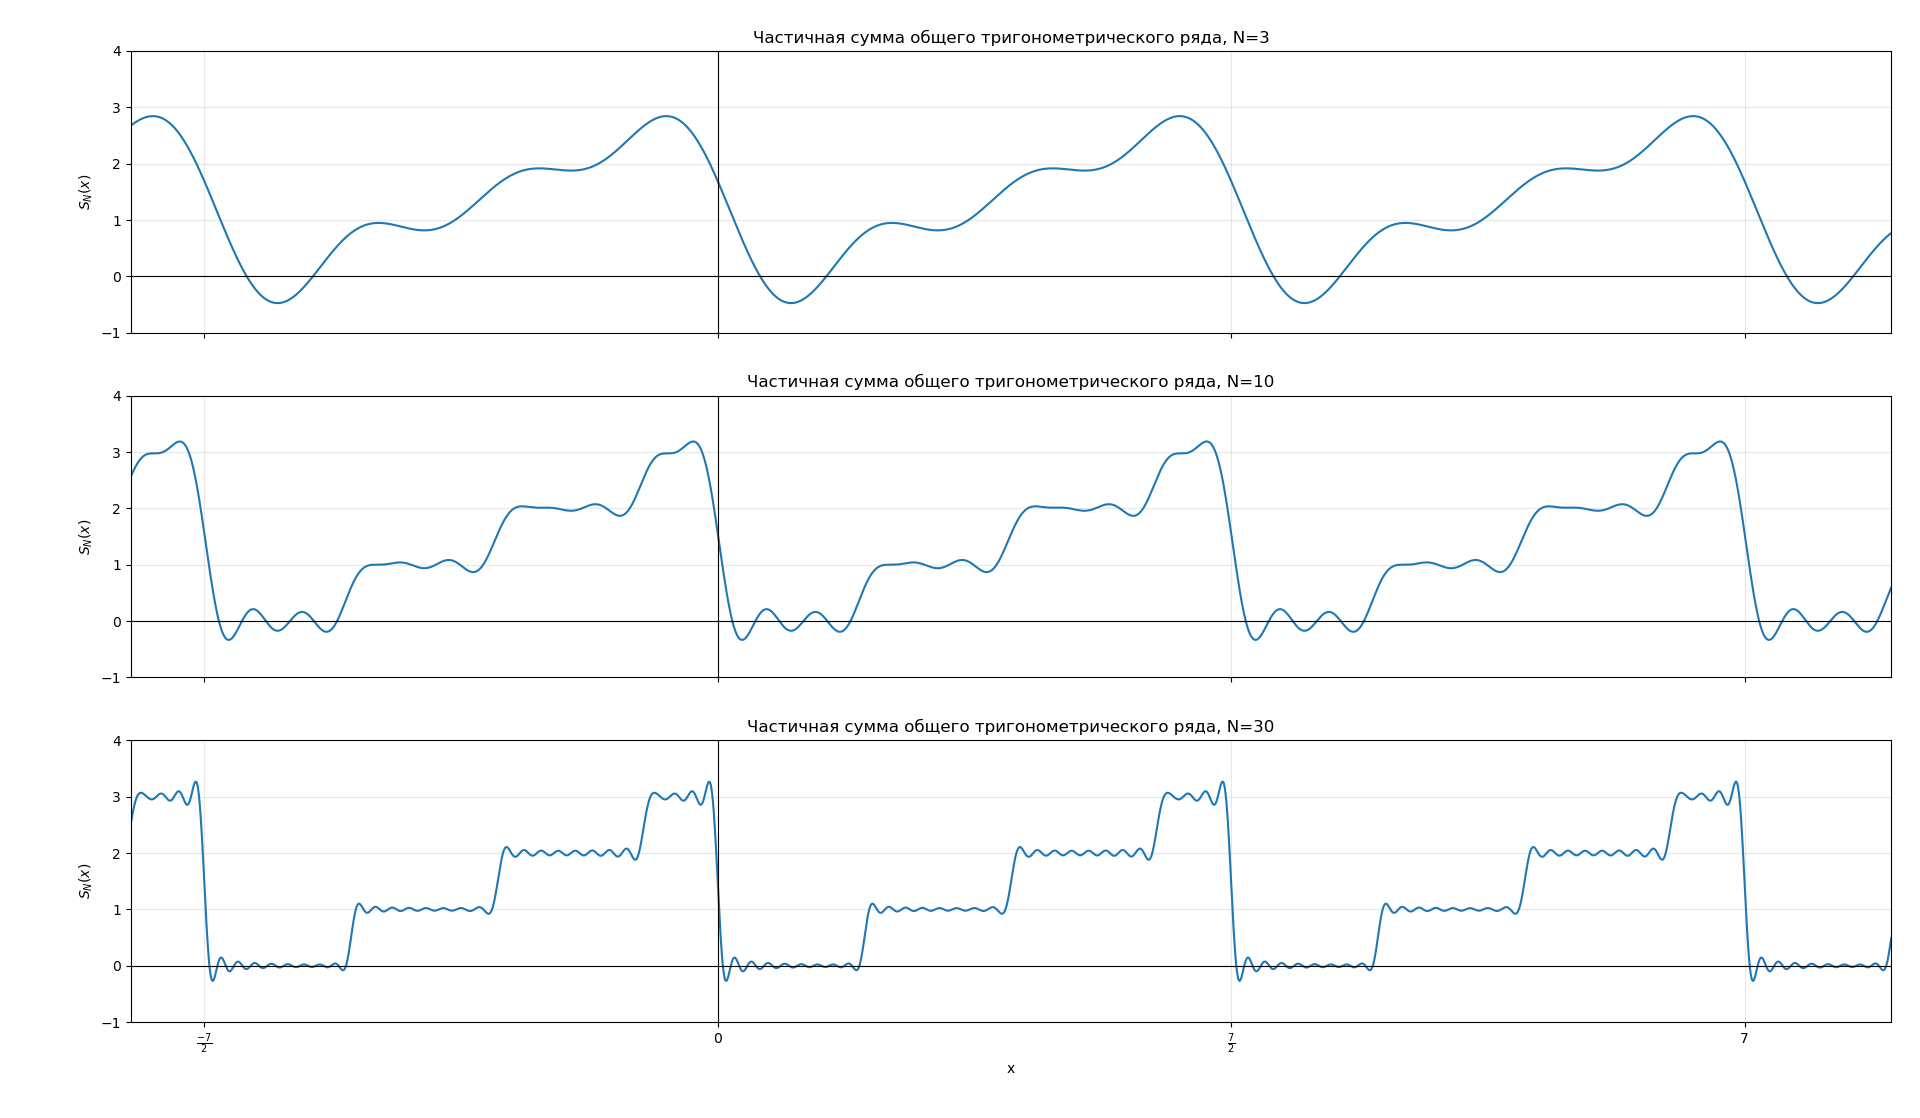
\includegraphics[width=1\textwidth]{../imgs/Figure_4.png}
    \caption{Графики частичных сумм общего тригонометрического ряда}
\end{figure}

\subsubsection*{Ряд по косинусам}

Для ряда Фурье по косинусам частичная сумма имеет вид
\[
S_{c,n}(x)=
\frac97
-
\sum_{k=1}^{n}
\frac2{\pi k}
\left(
\sin\frac{2\pi k}{7}
+
\sin\frac{4\pi k}{7}
+
\sin\frac{6\pi k}{7}
\right)
\cos\frac{2\pi kx}{7}
\]

\begin{figure}[H]
    \centering
    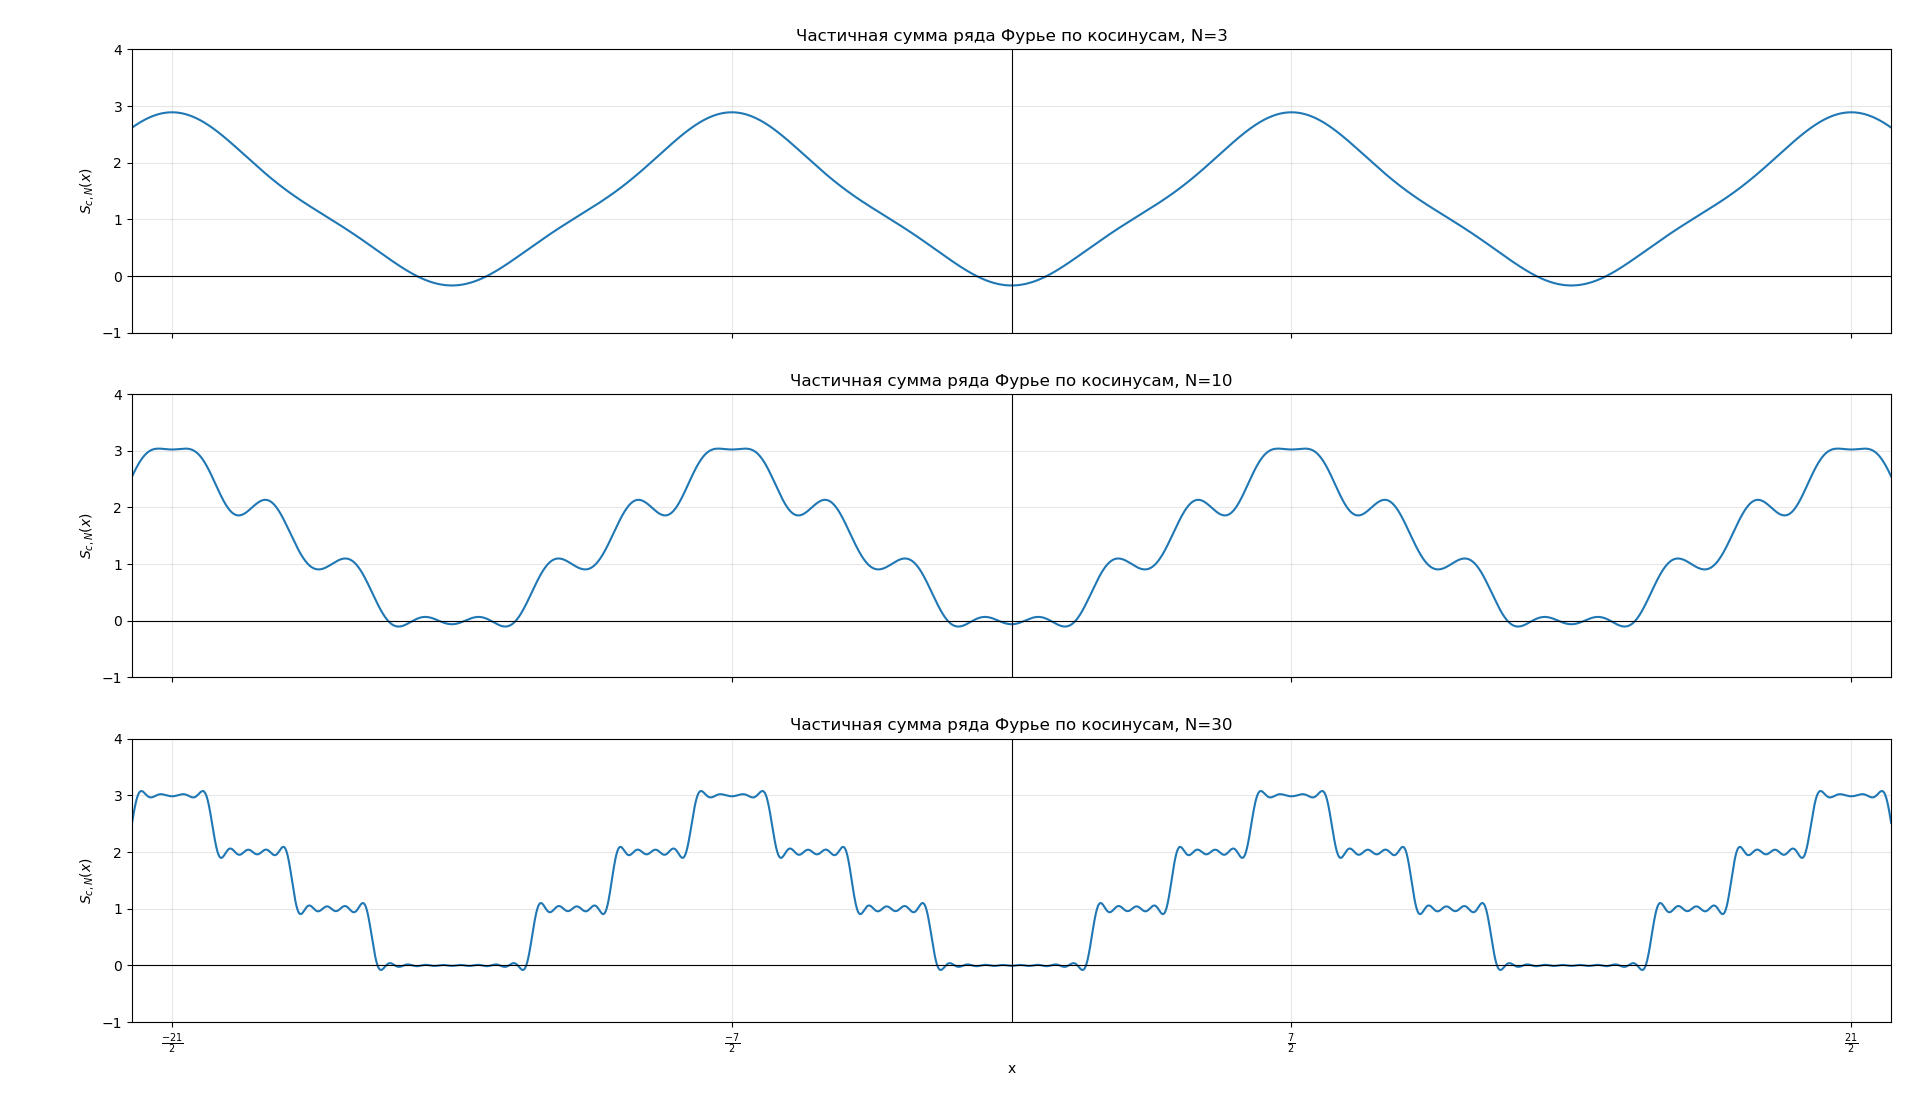
\includegraphics[width=1\textwidth]{../imgs/Figure_5.png}
    \caption{Графики частичных сумм ряда Фурье по косинусам}
\end{figure}

\subsubsection*{Ряд по синусам}

Для ряда Фурье по синусам частичная сумма имеет вид
\[
S_{s,n}(x)=
\sum_{k=1}^{n}
\frac2{\pi k}
\left(
\cos\frac{2\pi k}{7}
+
\cos\frac{4\pi k}{7}
+
\cos\frac{6\pi k}{7}
-
3(-1)^k
\right)
\sin\frac{2\pi kx}{7}.
\]

\begin{figure}[H]
    \centering
    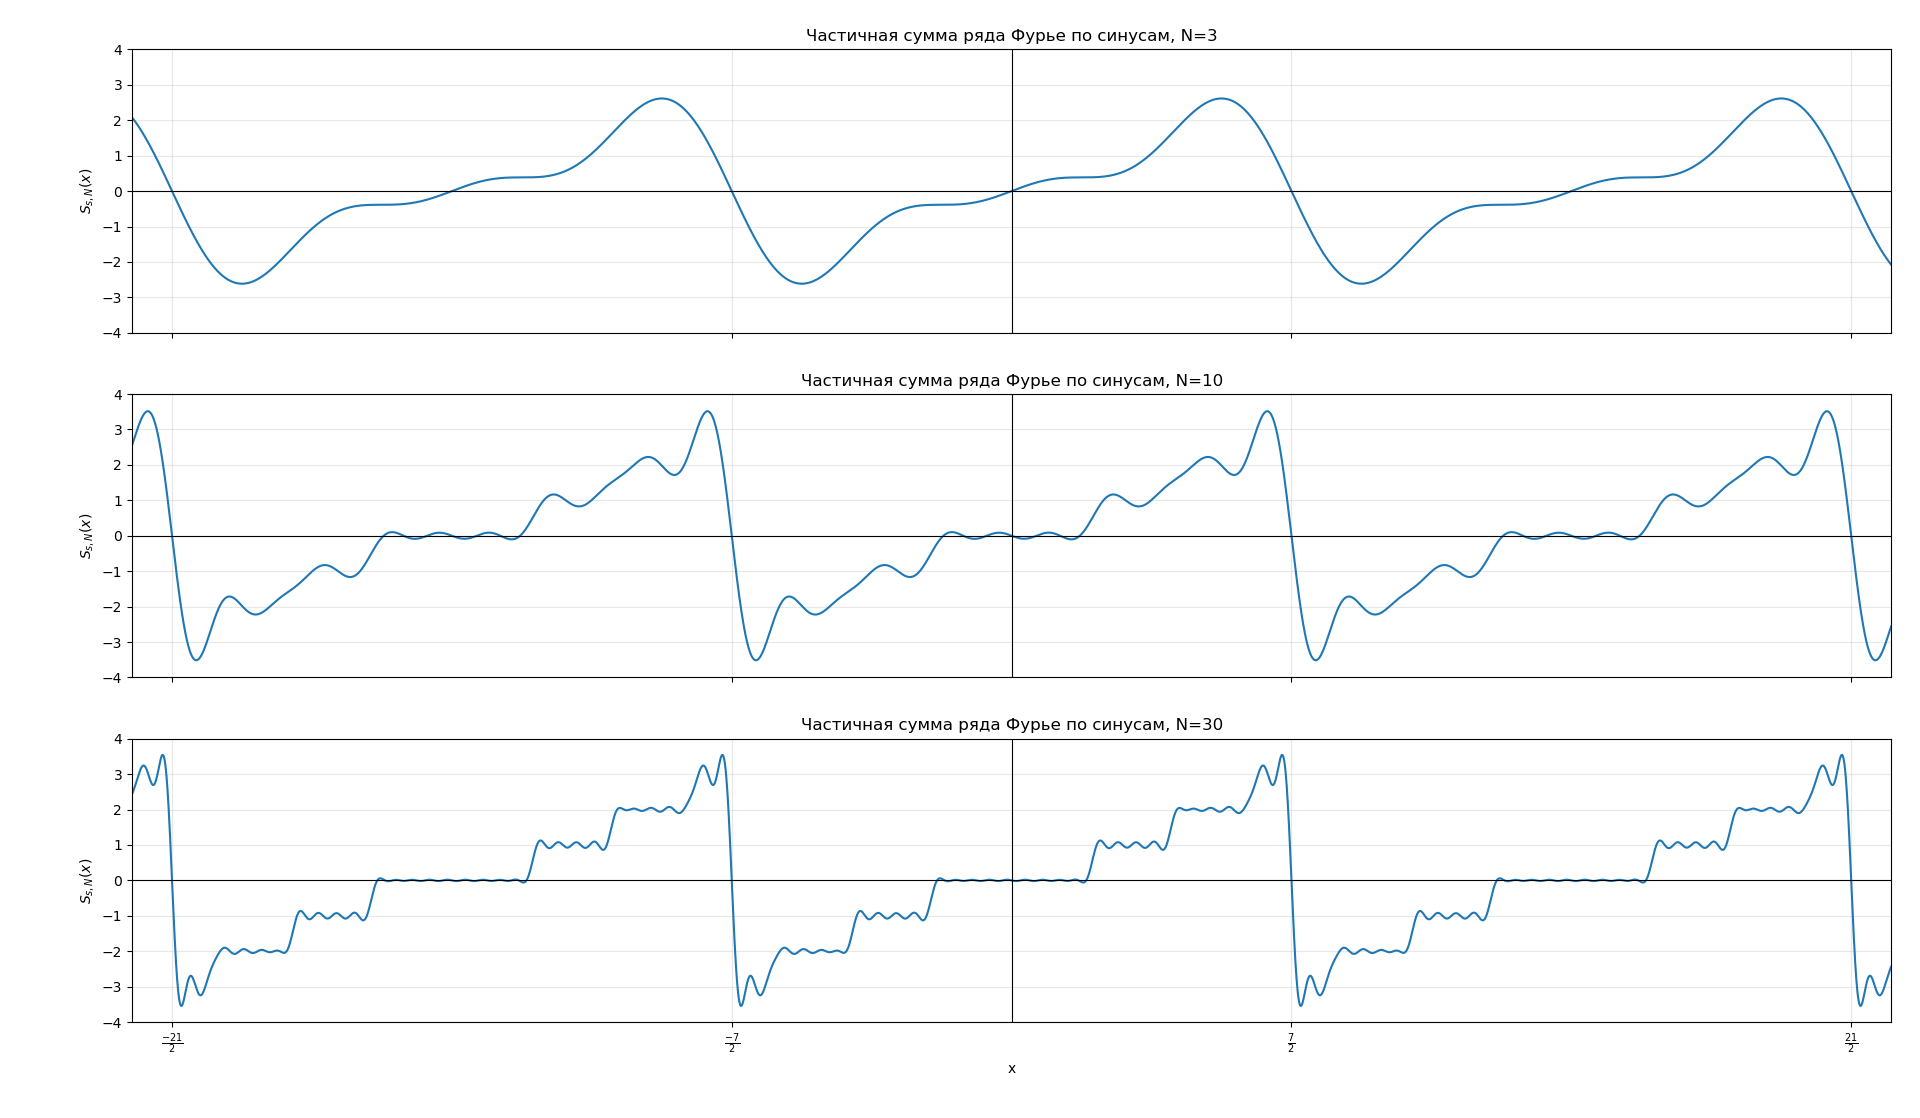
\includegraphics[width=1\textwidth]{../imgs/Figure_6.png}
    \caption{Графики частичных сумм ряда Фурье по синусам}
\end{figure}

\subsection{Выводы}

По построенным графикам видно, что при увеличении числа слагаемых \(N\)
частичные суммы всё лучше приближают графики сумм рядов, найденные в
аналитической части. Поэтому численный расчёт подтверждает полученные
формулы для рядов Фурье.

Совпадение происходит потому, что частичная сумма является приближением
того же самого ряда Фурье. При \(N\to\infty\) частичные суммы стремятся к
сумме ряда.

Связь между суммой ряда Фурье и исходной функцией задаётся теоремой
Дирихле. В точках непрерывности исходной функции сумма ряда совпадает со
значением функции:
\[
S(x)=f(x).
\]

В точках разрыва сумма ряда не равна ни левому, ни правому значению
функции. Она равна среднему арифметическому односторонних пределов:
\[
S(x_0)=
\frac{f(x_0-0)+f(x_0+0)}{2}.
\]

Таким образом, ряд Фурье восстанавливает исходную функцию в точках
непрерывности, а в точках скачка принимает значение, равное полусумме
левого и правого пределов. Для чётного и нечётного продолжений это
утверждение применяется уже к соответствующим продолженным функциям.

\end{document}
